% Copyright (c) 2021 Eclipse Arrowhead Project
%
% This program and the accompanying materials are made available under the
% terms of the Eclipse Public License 2.0 which is available at
% http://www.eclipse.org/legal/epl-2.0.
%
% SPDX-License-Identifier: EPL-2.0

There are eight certificate profiles defined in this document, depicted in the following diagram:

\begin{figure}[ht!]
  \centering
  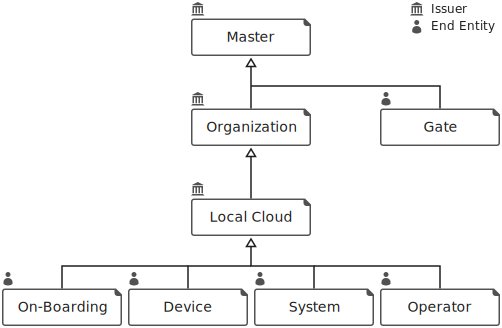
\includegraphics[scale=0.8]{figures/profile-hierarchy}
  \caption{
    Hierarchy of X.509 Profiles
  }
  \label{fig:profile-hierarchy}
\end{figure}

Each diagram box represents a profile.
The arrows in the diagram are to be read as "issued by", meaning that the every certificate adhering to the profile from which the arrow extends must be issued (signed) by a certificate with the profile pointed to.

In this section, we begin by considering the X.509 format itself, after which we outline the Master, Gate, Organization, Local Cloud, On-Boarding, Device, System and Operator profiles.
Each profile is described in terms of its (a) purpose, (b) issuer, (c) subject name and (d) extensions.
The details included in this section are intended to be enough to allow for the correct parameterization of certificates, but are unlikely to be sufficient for implementing software for handling them.
If the latter is relevant, please refer to RFC 5280, X.509, X.501, X.690 and ASN.1.

\subsection{Certificate Format}

The ASN.1 syntax of the third version of the X.509 certificate format is defined in as follows in RFC 5280:

\begin{verbatim}
    Certificate ::= SEQUENCE {
        tbsCertificate       TBSCertificate,
        signatureAlgorithm   AlgorithmIdentifier,
        signatureValue       BIT STRING
    }

    TBSCertificate ::= SEQUENCE {
        version         [0]  EXPLICIT Version DEFAULT v1,
        serialNumber         INTEGER,
        signature            AlgorithmIdentifier,
        issuer               Name,
        validity             Validity,
        subject              Name,
        subjectPublicKeyInfo SubjectPublicKeyInfo,
        issuerUniqueID  [1]  IMPLICIT UniqueIdentifier OPTIONAL,
        subjectUniqueID [2]  IMPLICIT UniqueIdentifier OPTIONAL,
        extensions      [3]  EXPLICIT Extensions OPTIONAL
    }
\end{verbatim}

The \texttt{Certificate} structure itself consists only of a \texttt{TBSCertificate}, a signature algorithm identifier and a concrete signature.
The signature is meant to be produced by the issuer of the certificate and serves to protect the integrity of the certificate under the assumption that the issuer is trusted.
All data protected by the signature is collected in the \texttt{TBSCertificate}, the fields of which are described in the following subsections.

\subsubsection{\texttt{version}}

X.509 version of the certificate.
Only \texttt{v3(2)} supports certificate extensions, which \textit{must} be used by all profiles described in this document.
Supporting \texttt{v1(0)} and \texttt{v2(1)} at all is \textit{optional}.

\subsubsection{\texttt{serialNumber}}

A positive integer of no more than 20 octets uniquely assigned by the issuer of the certificate.

\textbf{Security recommendation}.
The serial number should be exactly 20 octets long and be produced by a cryptographic random number generator.
This serves both to (A) make the certificate more resistant to collision attacks and (B) to prevent the serial number from leaking important details about the certificate issuer, such as how many certificates it has issued, how long the signing process took, and so on.
If certificate size would be a major concern, for example when certificates are used by significantly constrained devices, fewer octets \textit{may} be used.
Note that the serial number is signed and must be positive, which means that the most significant bit of its first ASN.1 BER \texttt{INTEGER} octet must be 0.

\subsubsection{\texttt{signature}}

Identifies the signature suite used to produce the \texttt{signatureValue} in the enclosing \texttt{Certificate}, as well as any parameters made relevant by the suite.
Examples of suites could be \textit{RSA with SHA256} or \textit{ED25519}.
This field must contain the same suite as the \texttt{signatureAlorithm} field in the enclosing \texttt{Certificate}, as described in the beginning of Section 2.1.

See Section 3 for information about selecting cryptographic algorithms.

\subsubsection{\texttt{issuer}}

The DN of the issuer of the certificate in question.
More specifically, this field contains an exact copy of the \texttt{subject} field of Section 2.1.6 from the certificate of its issuer, or a copy of the \texttt{issuer} field of the same certificate if it is self-signed.

\subsubsection{\texttt{validity}}

The period during which the certificate \textit{may} remain active and its issuer is bound to know whether or not the certificate has been revoked or not.
Denoted as a duration between two timestamps, \texttt{notBefore} and \texttt{notAfter}, as show below.

\begin{verbatim}
Validity ::= SEQUENCE {
    notBefore   Time,
    notAfter    Time
}

Time ::= CHOICE {
    utcTime     UTCTime,
    generalTime GeneralizedTime
}
\end{verbatim}

For each of these two dates, the date in question \textit{must} be encoded as a \texttt{UTCTime} if its year is less than or equal to 2049, or as a \texttt{GeneralizedTime} if the year is equal to or greater than 2050.
See Section 4.1.2.5 of RFC 5280 for more details.

The time span denoted by this field \textit{should} be shorter than the expected lifetime of the entity owning it, typically significantly shorter, if provisions exist for renewing it during its lifetime.
More specific recommendations will be published in other documents of the Eclipse Arrowhead project.

\subsubsection{\texttt{subject}}

The DN used to describe the owner of the certificate.
The field is defined as follows:

\begin{verbatim}
Name ::= CHOICE {
    rdnSequence RDNSequence
}

RDNSequence ::= SEQUENCE OF RelativeDistinguishedName

RelativeDistinguishedName ::= SET SIZE (1..MAX) OF AttributeTypeAndValue

AttributeTypeAndValue ::= SEQUENCE {
    type  AttributeType,
    value AttributeValue
}

AttributeType ::= OBJECT IDENTIFIER

-- Concrete type determined by associated \texttt{AttributeType}.
-- In our case that type will always be \texttt{DirectoryString}.
AttributeValue ::= ANY

DirectoryString ::= CHOICE {
     teletexString   TeletexString   (SIZE (1..MAX)),
     printableString PrintableString (SIZE (1..MAX)),
     universalString UniversalString (SIZE (1..MAX)),
     utf8String      UTF8String      (SIZE (1..MAX)),
     bmpString       BMPString       (SIZE (1..MAX)) 
}
\end{verbatim}

The below `AttributeType`s \textit{must} be supported by compliant software implementations, as required by RFC 5280.
Supporting them means that that their OIDs are known to be associated with values of type \texttt{DirectoryString}, as defined above.
Failing to support them means that the certificate validation procedure of RFC 5280, Section 6, cannot be executed.
See RFC 5280 Section 4.1.2.4 for more attributes that \textit{should} be supported.

\vspace*{0.5cm}
\noindent\begin{tabularx}{\textwidth}{| p{5cm} | p{3cm} | X |} \hline
\rowcolor{gray!33} Attribute Type & Abbreviation & OID \\ \hline

Common Name                       & \texttt{CN}  & \texttt{2.5.4.3} \\ \hline
Country                           & \texttt{C}   & \texttt{2.5.4.6}  \\ \hline
Distinguished Name Qualifier      & \texttt{DN}  & \texttt{2.5.4.46} \\ \hline
Domain Component                  & \texttt{DC}  & \texttt{0.9.2342.19200300.100.1.25} \\ \hline
Organization                      & \texttt{O}   & \texttt{2.5.4.10} \\ \hline
Organizational Unit               & \texttt{OU}  & \texttt{2.5.4.11} \\ \hline
Serial Number                     & \texttt{SN}  & \texttt{2.5.4.5} \\ \hline
State or Province Name            & \texttt{ST}  & \texttt{2.5.4.8} \\ \hline

\end{tabularx}
\vspace*{0.5cm}

Every certificate \textit{must} contain at least one \texttt{subject} \textit{Distinguished Name Qualifier} (\texttt{DN}).
It \textit{should} only contain one.
It \textit{should} be encoded as a \texttt{PrintableString}.
The rightmost (i.e. least significant) such identifies the profile of the certificate.
The identifiers are as follows:

\vspace*{0.5cm}
\noindent\begin{tabularx}{\textwidth}{| p{3cm} | X |} \hline
\rowcolor{gray!33} X.509 Profile  & Distinguished Name Qualifier (\texttt{DN}) \\ \hline

Master                            & \texttt{ma} \\ \hline
Gate                              & \texttt{ga} \\ \hline
Organization                      & \texttt{or} \\ \hline
Local Cloud                       & \texttt{lo} \\ \hline
On-Boarding                       & \texttt{on} \\ \hline
Device                            & \texttt{de} \\ \hline
System                            & \texttt{sy} \\ \hline
Operator                          & \texttt{op} \\ \hline

\end{tabularx}
\vspace*{0.5cm}

In addition, each certificate \textit{must} contain at least one \texttt{subject} \textit{Common Name} (\texttt{CN}) that is a valid DNS label (https://datatracker.ietf.org/doc/html/rfc1035\#section-2.3.1) of no more than 62 characters.
It \textit{should} only contain one \texttt{CN}.
It \textit{should} be encoded as a \texttt{PrintableString}.
The rightmost (i.e. least significant) such contains the name, or \textit{alias}, meant to be used by humans when referring to the certificate.
While names \textit{may} use up to 62 characters, we \textit{recommend} the use of 10 to 20 character long lowercase identifiers, such as \texttt{51e41vjoxq}, produced with secure random number generators.
Randomized identifiers hide details that otherwise would become accessible to adversaries with certificate copies, such as how many certificates have been issued, the type of machines they are associated with, and so on.
The \texttt{CN} field value \textit{must}, furthermore, be unique among all certificates issued by the same CA with same Distinguished Name Qualifier (\texttt{DN}).
It \textit{should not} be derived from a portion of the \texttt{serialNumber} of the same certificate.

The \texttt{CN} is meant to help humans refer to specific certificates, they \textit{should not} be used as primary references by machines.
See Section 4 for a discussion about machine certificate references.

\subsubsection{\texttt{subjectPublicKeyInfo}}

The public key of the subject, as well as the identity of the algorithm associated with it.
The field is defined as follows.

\begin{verbatim}
SubjectPublicKeyInfo ::= SEQUENCE {
    algorithm        AlgorithmIdentifier,
    subjectPublicKey BIT STRING
}
\end{verbatim}

See Section 3 for information about selecting cryptographic algorithms.

\subsubsection{\texttt{issuerUniqueID} and \texttt{subjectUniqueID}}

Optional identifiers uniquely associated with the issuer or subject of the certificate.

These fields \textit{must not} be used.
See Section 4 for a discussion about certificate identification.

\subsubsection{\texttt{extensions}}

A list of certificate extensions, as defined below.

\begin{verbatim}
Extensions ::= SEQUENCE SIZE (1..MAX) OF Extension

Extension  ::= SEQUENCE {
    extnID     OBJECT IDENTIFIER,
    critical   BOOLEAN DEFAULT FALSE,
    extnValue  OCTET STRING
}
\end{verbatim}

RFC 5280 explicitly outlines 17 different X.509 extensions, listed by category below.

\vspace*{0.35cm}
\noindent\begin{tabularx}{\textwidth}{| p{4.5cm} | p{2.3cm} | X |} \hline
\rowcolor{gray!33} Extension    & \texttt{extnID} (OID) & Brief Description \\ \hline

\multicolumn{3}{| l |}{\textbf{Identifier Extensions}} \\ \hline
Authority Key Identifier        & \texttt{2.5.29.35}          & Identifier uniquely associated with certificate issuer. \\ \hline
Subject Key Identifier          & \texttt{2.5.29.14}          & Identifier uniquely associated with certificate subject. \\ \hline
\multicolumn{3}{| l |}{\textbf{Key Usage Extensions}} \\ \hline
Key Usage                       & \texttt{2.5.29.15}          & Public key usage restrictions. \\ \hline
Extended Key Usage              & \texttt{2.5.29.37}          & Additional public key usage restrictions. \\ \hline
\multicolumn{3}{| l |}{\textbf{Policy Extensions}} \\ \hline
Certificate Policies            & \texttt{2.5.29.32}          & List of policies accepted by the certificate subject. \\ \hline
Policy Mappings                 & \texttt{2.5.29.33}          & List of policy equivalence relations. \\ \hline
Policy Constraints              & \texttt{2.5.29.36}          & Policy validation constraints (e.g. policy X must be accepted). \\ \hline
Inhibit \texttt{anyPolicy}      & \texttt{2.5.29.54}          & Policy validation constraint related to use of \texttt{anyPolicy}. \\ \hline
\multicolumn{3}{| l |}{\textbf{Name Extensions}} \\ \hline
Subject Alternative Name        & \texttt{2.5.29.17}          & Additional names associated with the certificate subject. \\ \hline
Issuer Alternative Name         & \texttt{2.5.29.18}          & Additional names associated with the certificate issuer. \\ \hline
Name Constraints                & \texttt{2.5.29.30}          & List of subject name restrictions for issued certificates. \\ \hline
\multicolumn{3}{| l |}{\textbf{CRL Extensions}} \\ \hline
CRL Distribution Points         & \texttt{2.5.29.31}          & List of where relevant CRLs can be found. \\ \hline
Freshest CRL                    & \texttt{2.5.29.46}          & List of where delta CRLs can be found. \\ \hline
\multicolumn{3}{| l |}{\textbf{Information Extensions}} \\ \hline
Authority Information Access    & \texttt{1.3.6.1.5. 5.7.1.1}  & List of where issuer information and services can be found. \\ \hline
Subject Information Access      & \texttt{1.3.6.1.5. 5.7.1.11} & List of where subject information and services can be found. \\ \hline
\multicolumn{3}{| l |}{\textbf{Other Extensions}} \\ \hline
Subject Directory Attributes    & \texttt{2.5.29.9}           & Additional subject identification attributes (e.g. nationality). \\ \hline
Basic Constraints               & \texttt{2.5.29.19}          & Description of where a certificate belongs in its CA hierarchy. \\ \hline

\end{tabularx}
\vspace*{0.35cm}

Each category of extensions is described in the following subsections.

\paragraph{Identifier Extensions}

The \textbf{Authority Key Identifier} and \textbf{Subject Key Identifier} extensions are used to identify the public key of the issuer and subject of a given certificate, respectively.
The extensions are defined as follows:

\begin{verbatim}
-- Required for all but self-signed CA certificates (root CAs).
AuthorityKeyIdentifier ::= SEQUENCE {
    keyIdentifier             [0] KeyIdentifier           OPTIONAL, -- Required.
    authorityCertIssuer       [1] GeneralNames            OPTIONAL, -- Should not be used.
    authorityCertSerialNumber [2] CertificateSerialNumber OPTIONAL  -- Should not be used.
}

-- Required for all but end entity certificates.
SubjectKeyIdentifier ::= KeyIdentifier

KeyIdentifier ::= OCTET STRING
\end{verbatim}

RFC 5280 \textit{requires} that \texttt{AuthorityKeyIdentifier} extension is included in all CA certificates except for self-signed such.
The \texttt{keyIdentifier} of the \texttt{AuthorityKeyIdentifier} extension of a given certificate \textit{must} match the \texttt{SubjectKeyIdentifier} of its issuer's certificate, or \textit{may} be omitted if the certificate is self-signed.
Use of the \texttt{authorityCertIssuer} and \texttt{authorityCertSerialNumber} fields of \texttt{AuthorityKeyIdentifier} is \textit{not recommended}.
If a self-signed certificate leaves the \texttt{authorityCertIssuer} and \texttt{authorityCertSerialNumber} fields unspecified, it may omit the \texttt{AuthorityKeyIdentifier} extension entirely.
RFC 5280 further \textit{requires} that all but end entity certificates use the \texttt{SubjectKeyIdentifier} extension.
Its value \textit{should} be the the cryptographic hash of the \texttt{subjectPublicKey} value (excluding the tag, length, and number of unused bits) of the \texttt{subjectPublicKeyInfo} field.
See Section 3 for a discussion about what hash algorithms to use.
The extensions \textit{must not} be marked as critical.

\paragraph{Key Usage Extensions}

The \textbf{Key Usage} and \textbf{Extended Key Usage} extensions are defined as follows:

\begin{verbatim}
KeyUsage ::= BIT STRING {
    digitalSignature (0),
    nonRepudiation   (1), -- Also known as \texttt{contentCommitment}.
    keyEncipherment  (2),
    dataEncipherment (3),
    keyAgreement     (4),
    keyCertSign      (5),
    cRLSign          (6),
    encipherOnly     (7),
    decipherOnly     (8)
}

ExtKeyUsageSyntax ::= SEQUENCE SIZE (1..MAX) OF KeyPurposeId

KeyPurposeId ::= OBJECT IDENTIFIER
\end{verbatim}

The \texttt{KeyUsage} extension is a set of bit flags indicating various ways in which a certificate \textit{must} only be used.
Please refer to RFC 5280 Section 4.2.1.3 for descriptions of each bit flag.
The extension \textit{must} be used in all certificates and \textit{must} be marked as critical.
How to set it is outlined in the section specific to each particular certificate profile.

The \texttt{ExtKeyUsageSyntax} extension has the same purpose, but is open-ended in the sense that it allows for any OID to be used as an indication of what a certain certificate \textit{may} be used for.
RFC 5280 lists six such purpose identifiers, out of which two has particular bearing on this document, namely the \texttt{serverAuth} (OID \texttt{1.3.6.1.5.5.7.3.1}) and \texttt{clientAuth} (OID \texttt{1.3.6.1.5.5.7.3.2}) identifiers, which indicate that the certificate holder must be able to respond to TLS server and client authorization requests, respectively.
The extension \textit{must} be used in all end entity certificates, as well in the certificates of the CAs that handle CSRs directly via network application interfaces.
The \texttt{serverAuth} and \texttt{clientAuth} identifiers \textit{must} be included.
The extension \textit{should not} be marked as \textit{critical}.
Other purpose identifiers \textit{may} be used.

\paragraph{Policy Extensions}

In the context of X.509 and RFC 5280, a \textit{policy} is a legal document that binds the owner of a certificate, and, potentially, all certificates issued by that certificate, to certain legal obligations.
The four policy extensions defined by RFC 5280 \textit{may} be used to ensure that every certificate in a given certificate chain have accepted some policies of concern.
Please refer to RFC 5280 for more details about these extensions.

\paragraph{Name Extensions}

The \textbf{Subject Alternative Name} and \textbf{Issuer Alternative Name} allows for additional identities to be associated with a given \texttt{subject} or \texttt{issuer} name.
Such additional identities significantly include DNS names, IP addresses and e-mail addresses.
For example, given that some system receives a signed message and the certificate associated with that signature, the system can verify that it received the message via one of the identities listed as subject alternative name in that certificate.
The extensions are defined as follows:

\begin{verbatim}
SubjectAltName ::= GeneralNames
IssuerAltName  ::= GeneralNames

GeneralNames ::= SEQUENCE SIZE (1..MAX) OF GeneralName

GeneralName ::= CHOICE {
    otherName                 [0] OtherName,
    rfc822Name                [1] IA5String,
    dNSName                   [2] IA5String,
    x400Address               [3] ORAddress,
    directoryName             [4] Name,
    ediPartyName              [5] EDIPartyName,
    uniformResourceIdentifier [6] IA5String,
    iPAddress                 [7] OCTET STRING,
    registeredID              [8] OBJECT IDENTIFIER
}
\end{verbatim}

The \texttt{SubjectAltName} extension \textit{must} be used by all end entity certificates and \textit{must} identify at least one DNS name, IP address or other relevant identifier useful for contacting the certificate owner.
The extension \textit{must} also be used for CA certificates that handles CSRs directly via network application interfaces.
Use of the \texttt{IssuerAltName} is \textit{not recommended}.
Both extensions \textit{should} be marked as non-critical.

\textbf{Security recommendation}.
All names appearing in a \texttt{SubjectAltName} extension \textit{should} be randomized, by which we mean that every name is formulated such that an adversary can derive as little information as possible from it.
In the case of an IP address, this means that a larger address space is preferred (e.g. 10.0.0.0/8 rather than 192.168.0.0/16) and that addresses are assigned randomly rather than sequentially.
In the case of DNS names, this means that no serially assigned identifiers are used and that no human-readable descriptors of sensitive places or things are part of the name.
See Section 7 for a discussion about the use of DNS in the context of Arrowhead.

The \textbf{Name Constraints} extension makes it possible for a CA to restrict the set of values allowed for the \texttt{subject} and \texttt{SubjectAltName} fields in issued certificates.
The extension \textit{should not} be used.
It \textit{must} be marked as critical if used.
Please refer to RFC 5280 Section 4.2.1.10 for more details.

\paragraph{CRL Extensions}

The CRL extensions facilitate a mechanism for revoking certificates that are still valid and distributing information about those revocations.
These extensions \textit{should not} be used to facilitate the revocation of On-Boarding, Device, System and Operator certificates.
They \textit{may} be used for revoking certificates of the other profiles.

Eclipse Arrowhead comes with its own certificate revocation procedure via its \textit{Certificate Authority} system.
Its use is \textit{recommended} for revoking and verifying the validity of On-Boarding, Device, System and Operator certificates.

\paragraph{Information Extensions}

The information extensions allows for various types of data sources or services to be associated with the certificate holder.
These extensions \textit{should not} be used, unless required by a protocol relevant for the revocation of Master, Organization, Gate and Local Cloud certificates.

Eclipse Arrowhead has its own provisions for metadata distribution and service management, via the \textit{Service Registry} system, \textit{Gatekeeper} system, and other.
Those provisions \textit{should} be used.

\paragraph{Other Extensions}

The \textbf{Subject Directory Attributes} allows for arbitrary identification attributes, such as nationality, to be associated with the \texttt{subject} of a certificate.
It \textit{may} be used.
It \textit{must} be marked as non-critical if used.

The \textbf{Basic Constraints} extension allows for it to be denoted whether or not a given certificate belongs to a CA, as well as how many intermediary CAs may exist below it in any given certificate chain.
The extension is defined as follows:

\newpage

\begin{verbatim}
BasicConstraints ::= SEQUENCE {
    cA                BOOLEAN DEFAULT FALSE,
    pathLenConstraint INTEGER (0..MAX) OPTIONAL
}
\end{verbatim}

The extension \textit{must} be used and marked critical by all Arrowhead-compliant certificates.
The \texttt{pathLenConstraint} \textit{must} be set by all CA certificates, but \textit{must not} be set by end entity certificates.

\newpage
\subsection{Master Profile}

A \textit{Master} certificate exists to establish trust between organizations that may want to interconnect their Arrowhead systems.
It does this by issuing \textit{Organization} and \textit{Gate} certificates.
The former enables organizations to set up their own certificate hierarchies while sharing a common CA with other organizations.
The latter kind enables all those organizations to trust a special kind of broker system, which facilitates negotiating connections between organizations.

The Eclipse Arrowhead project \textit{should} maintain an authoritative Master certificate that \textit{may} be used for non-private Arrowhead installations.
Other entities \textit{may} setup and maintain their own Master certificates as needed.

\subsubsection{\texttt{issuer}}

\textit{May} be self-signed or issued by an RFC 5280-compliant CA.

\textbf{Security notice}.
In the case of a Master being issued by a widely trusted World Wide Web CA, entities with the Master in their certificate chains could be made able to serve HTTP(S) traffic to regular web browsers without any additional certificate distribution.
It could also make it possible for improperly configured systems to establish secure connections with unauthorized systems.
Having CAs above a Master provides for new opportunities and new risks at the same time, for which reason it may or may not be desirable.

\subsubsection{\texttt{subject}}

The subject field DN \textit{must} contain the following attributes exactly once, either in the same or different RDNs:

\vspace*{0.5cm}
\noindent\begin{tabularx}{\textwidth}{| p{4cm} | p{2cm} | X |} \hline
\rowcolor{gray!33} Attribute Type & OID               & Value \\ \hline

DN Qualifier (DN)                 & \texttt{2.5.4.46} & \texttt{ma} \\ \hline
Common Name (CN)                  & \texttt{2.5.4.3}  &  Randomized identifier. See Section 2.1.6. \\ \hline

\end{tabularx}
\vspace*{0.5cm}


\subsubsection{\texttt{extensions}}

The following extensions \textit{must} be used and configured as described:

\vspace*{0.5cm}
\noindent\begin{tabularx}{\textwidth}{| p{4cm} | p{2cm} | p{1.2cm} | X |} \hline
\rowcolor{gray!33} Extension & OID                & Critical & Value \\ \hline

Authority Key Identifier     & \texttt{2.5.29.35} & No       & Hash of issuer public key. Omit field if self-signed. See Section 2.1.9.1. \\ \hline
Subject Key Identifier       & \texttt{2.5.29.14} & No       & Hash of subject public key. See Section 2.1.9.1. \\ \hline
Basic Constraints            & \texttt{2.5.29.19} & Yes      & \texttt{cA: true, pathLenConstraint: 2}. See Section 2.1.9.7. \\ \hline
Key Usage                    & \texttt{2.5.29.15} & Yes      & Bits \texttt{keyCertSign(5)} and \texttt{cRLSign(6)} \textit{must} be set. See Section 2.1.9.2. \\ \hline

\end{tabularx}
\vspace*{0.5cm}

If the certificate will be used to automatically respond to CSRs via a network application interface, the following must also be present:

\vspace*{0.5cm}
\noindent\begin{tabularx}{\textwidth}{| p{4cm} | p{2cm} | p{1.2cm} | X |} \hline
\rowcolor{gray!33} Extension & OID                & Critical & Value \\ \hline

Key Usage                    & \texttt{2.5.29.15} & Yes      & Bits \texttt{digitalSignature(0)} and \texttt{keyEncipherment(2)} \textit{must} be set in addition to \texttt{5} and \texttt{6}. See Section 2.1.9.2. \\ \hline
Extended Key Usage           & \texttt{2.5.29.37} & No       & Purposes`serverAuth` and \texttt{clientAuth} \textit{must} be specified. See Section 2.1.9.2. \\ \hline
Subject Alternative Name     & \texttt{2.5.29.17} & No       & At least one IP address, DNS name or other identifier to which CSRs can be sent. See Section 2.1.9.4. \\ \hline

\end{tabularx}
\vspace*{0.5cm}

\newpage
\subsection{Gate Profile}

A \textit{Gate} certificate is associated with a message broker or bus that exists to guarantee delivery of messages between the local clouds of distinct organizations.
Its existence means that such messages can sent over a secure transport.

\subsubsection{\texttt{issuer}}

\textit{Must} be issued by a Master certificate.

\subsubsection{\texttt{subject}}

The subject field DN \textit{must} contain the following attributes exactly once, either in the same or different RDNs:

\vspace*{0.5cm}
\noindent\begin{tabularx}{\textwidth}{| p{4cm} | p{2cm} | X |} \hline
\rowcolor{gray!33} Attribute Type & OID               & Value \\ \hline

DN Qualifier (DN)                 & \texttt{2.5.4.46} & \texttt{ga} \\ \hline
Common Name (CN)                  & \texttt{2.5.4.3}  &  Randomized identifier. See Section 2.1.6. \\ \hline

\end{tabularx}
\vspace*{0.5cm}

\subsubsection{\texttt{extensions}}

The following extensions \textit{must} be used and configured as described:

\vspace*{0.5cm}
\noindent\begin{tabularx}{\textwidth}{| p{4cm} | p{2cm} | p{1.2cm} | X |} \hline
\rowcolor{gray!33} Extension & OID                & Critical & Value \\ \hline

Authority Key Identifier     & \texttt{2.5.29.35} & No       & Hash of issuer public key. See Section 2.1.9.1. \\ \hline
Basic Constraints            & \texttt{2.5.29.19} & Yes      & \texttt{cA: false}. See Section 2.1.9.7. \\ \hline
Key Usage                    & \texttt{2.5.29.15} & Yes      & Bits \texttt{digitalSignature(0)} and \texttt{keyEncipherment(2)} \textit{must} be set. See Section 2.1.9.2. \\ \hline
Extended Key Usage           & \texttt{2.5.29.37} & No       & Purposes \texttt{serverAuth} and \texttt{clientAuth} \textit{must} be specified. See Section 2.1.9.2. \\ \hline
Subject Alternative Name     & \texttt{2.5.29.17} & No       & At least one IP address, DNS name or other identifier through which the system can be reached. See Section 2.1.9.4. \\ \hline

\end{tabularx}
\vspace*{0.5cm}

\newpage
\subsection{Organization Profile}

An \textit{Organization} certificate is maintained by a single organization, allowing it to manage the certificates of its own local clouds.

\subsubsection{\texttt{issuer}}

\textit{Must} be issued by a Master certificate.

\subsubsection{\texttt{subject}}

The subject field DN \textit{must} contain the following attributes exactly once, either in the same or different RDNs:

\vspace*{0.5cm}
\noindent\begin{tabularx}{\textwidth}{| p{4cm} | p{2cm} | X |} \hline
\rowcolor{gray!33} Attribute Type & OID               & Value \\ \hline

DN Qualifier (DN)                 & \texttt{2.5.4.46} & \texttt{or} \\ \hline
Common Name (CN)                  & \texttt{2.5.4.3}  &  Randomized identifier. See Section 2.1.6. \\ \hline

\end{tabularx}
\vspace*{0.5cm}

\subsubsection{\texttt{extensions}}

The following extensions \textit{must} be used and configured as described:

\vspace*{0.5cm}
\noindent\begin{tabularx}{\textwidth}{| p{4cm} | p{2cm} | p{1.2cm} | X |} \hline
\rowcolor{gray!33} Extension & OID                & Critical & Value \\ \hline

Authority Key Identifier     & \texttt{2.5.29.35} & No       & Hash of issuer public key. See Section 2.1.9.1. \\ \hline
Subject Key Identifier       & \texttt{2.5.29.14} & No       & Hash of subject public key. See Section 2.1.9.1. \\ \hline
Basic Constraints            & \texttt{2.5.29.19} & Yes      & \texttt{cA: true, pathLenConstraint: 1}. See Section 2.1.9.7. \\ \hline
Key Usage                    & \texttt{2.5.29.15} & Yes      & Bits \texttt{keyCertSign(5)} and \texttt{cRLSign(6)} \textit{must} be set. See Section 2.1.9.2. \\ \hline

\end{tabularx}
\vspace*{0.5cm}

If the certificate will be used to automatically respond to CSRs via a network application interface, the following must also be present:

\vspace*{0.5cm}
\noindent\begin{tabularx}{\textwidth}{| p{4cm} | p{2cm} | p{1.2cm} | X |} \hline
\rowcolor{gray!33} Extension & OID                & Critical & Value \\ \hline

Key Usage                    & \texttt{2.5.29.15} & Yes      & Bits \texttt{digitalSignature(0)} and \texttt{keyEncipherment(2)} \textit{must} be set in addition to \texttt{5} and \texttt{6}. See Section 2.1.9.2. \\ \hline
Extended Key Usage           & \texttt{2.5.29.37} & No       & Purposes`serverAuth` and \texttt{clientAuth} \textit{must} be specified. See Section 2.1.9.2. \\ \hline
Subject Alternative Name     & \texttt{2.5.29.17} & No       & At least one IP address, DNS name or other identifier to which CSRs can be sent. See Section 2.1.9.4. \\ \hline

\end{tabularx}
\vspace*{0.5cm}

\newpage
\subsection{Local Cloud Profile}

An \textit{Local Cloud} certificate is maintained by a single local cloud, enabling it to issue end entity certificates for on-boarding and on-boarded devices, as well as for systems and operators.

\subsubsection{\texttt{issuer}}

\textit{Must} be issued by an Organization certificate.

\subsubsection{\texttt{subject}}

The subject field DN \textit{must} contain the following attributes exactly once, either in the same or different RDNs:

\vspace*{0.5cm}
\noindent\begin{tabularx}{\textwidth}{| p{4cm} | p{2cm} | X |} \hline
\rowcolor{gray!33} Attribute Type & OID               & Value \\ \hline

DN Qualifier (DN)                 & \texttt{2.5.4.46} & \texttt{lo} \\ \hline
Common Name (CN)                  & \texttt{2.5.4.3}  &  Randomized identifier. See Section 2.1.6. \\ \hline

\end{tabularx}
\vspace*{0.5cm}

\subsubsection{\texttt{extensions}}

The following extensions \textit{must} be used and configured as described:

\vspace*{0.5cm}
\noindent\begin{tabularx}{\textwidth}{| p{4cm} | p{2cm} | p{1.2cm} | X |} \hline
\rowcolor{gray!33} Extension & OID                & Critical & Value \\ \hline

Authority Key Identifier     & \texttt{2.5.29.35} & No       & Hash of issuer public key. See Section 2.1.9.1. \\ \hline
Subject Key Identifier       & \texttt{2.5.29.14} & No       & Hash of subject public key. See Section 2.1.9.1. \\ \hline
Basic Constraints            & \texttt{2.5.29.19} & Yes      & \texttt{cA: true, pathLenConstraint: 0}. See Section 2.1.9.7. \\ \hline
Key Usage                    & \texttt{2.5.29.15} & Yes      & Bits \texttt{keyCertSign(5)} and \texttt{cRLSign(6)} \textit{must} be set. See Section 2.1.9.2. \\ \hline

\end{tabularx}
\vspace*{0.5cm}

If the certificate will be used to automatically respond to CSRs via a network application interface, the following must also be present:

\vspace*{0.5cm}
\noindent\begin{tabularx}{\textwidth}{| p{4cm} | p{2cm} | p{1.2cm} | X |} \hline
\rowcolor{gray!33} Extension & OID                & Critical & Value \\ \hline

Key Usage                    & \texttt{2.5.29.15} & Yes      & Bits \texttt{digitalSignature(0)} and \texttt{keyEncipherment(2)} \textit{must} be set in addition to \texttt{5} and \texttt{6}. See Section 2.1.9.2. \\ \hline
Extended Key Usage           & \texttt{2.5.29.37} & No       & Purposes`serverAuth` and \texttt{clientAuth} \textit{must} be specified. See Section 2.1.9.2. \\ \hline
Subject Alternative Name     & \texttt{2.5.29.17} & No       & At least one IP address, DNS name or other identifier to which CSRs can be sent. See Section 2.1.9.4. \\ \hline

\end{tabularx}
\vspace*{0.5cm}

\newpage
\subsection{On-Boarding Profile}

An \textit{On-Boarding} certificate allows for a device in an Arrowhead local cloud to request a new device certificate.
It is used both or either to provision new devices and/or to facilitate renewal of certificates as they are about to expire.
Certificates adhering to this profile \textit{must} only be provided to devices known or assumed to be trustworthy.

\subsubsection{\texttt{issuer}}

\textit{Must} be issued by a Local Cloud certificate.

\subsubsection{\texttt{subject}}

The subject field DN \textit{must} contain the following attributes exactly once, either in the same or different RDNs:

\vspace*{0.5cm}
\noindent\begin{tabularx}{\textwidth}{| p{4cm} | p{2cm} | X |} \hline
\rowcolor{gray!33} Attribute Type & OID               & Value \\ \hline

DN Qualifier (DN)                 & \texttt{2.5.4.46} & \texttt{on} \\ \hline
Common Name (CN)                  & \texttt{2.5.4.3}  &  Randomized identifier. See Section 2.1.6. \\ \hline

\end{tabularx}
\vspace*{0.5cm}

\subsubsection{\texttt{extensions}}

The following extensions \textit{must} be used and configured as described:

\vspace*{0.5cm}
\noindent\begin{tabularx}{\textwidth}{| p{4cm} | p{2cm} | p{1.2cm} | X |} \hline
\rowcolor{gray!33} Extension & OID                & Critical & Value \\ \hline

Authority Key Identifier     & \texttt{2.5.29.35} & No       & Hash of issuer public key. See Section 2.1.9.1. \\ \hline
Basic Constraints            & \texttt{2.5.29.19} & Yes      & \texttt{cA: false}. See Section 2.1.9.7. \\ \hline
Key Usage                    & \texttt{2.5.29.15} & Yes      & Bits \texttt{digitalSignature(0)} and \texttt{keyEncipherment(2)} \textit{must} be set. See Section 2.1.9.2. \\ \hline
Extended Key Usage           & \texttt{2.5.29.37} & No       & Purposes \texttt{serverAuth} and \texttt{clientAuth} \textit{must} be specified. See Section 2.1.9.2. \\ \hline
Subject Alternative Name     & \texttt{2.5.29.17} & No       & At least one IP address, DNS name or other identifier through which the owning device can be reached. See Section 2.1.9.4. \\ \hline

\end{tabularx}
\vspace*{0.5cm}

\newpage
\subsection{Device Profile}

A \textit{Device} certificate allows for a device in an Arrowhead local cloud to request new system certificates.
One system certificate is required for each system a given device intends to run.
Certificates adhering to this profile \textit{must} only be provided to devices known or assumed to be trustworthy.

\subsubsection{\texttt{issuer}}

\textit{Must} be issued by a Local Cloud certificate.

\subsubsection{\texttt{subject}}

The subject field DN \textit{must} contain the following attributes exactly once, either in the same or different RDNs:

\vspace*{0.5cm}
\noindent\begin{tabularx}{\textwidth}{| p{4cm} | p{2cm} | X |} \hline
\rowcolor{gray!33} Attribute Type & OID               & Value \\ \hline

DN Qualifier (DN)                 & \texttt{2.5.4.46} & \texttt{de} \\ \hline
Common Name (CN)                  & \texttt{2.5.4.3}  &  Randomized identifier. See Section 2.1.6. \\ \hline

\end{tabularx}
\vspace*{0.5cm}

\subsubsection{\texttt{extensions}}

The following extensions \textit{must} be used and configured as described:

\vspace*{0.5cm}
\noindent\begin{tabularx}{\textwidth}{| p{4cm} | p{2cm} | p{1.2cm} | X |} \hline
\rowcolor{gray!33} Extension & OID                & Critical & Value \\ \hline

Authority Key Identifier     & \texttt{2.5.29.35} & No       & Hash of issuer public key. See Section 2.1.9.1. \\ \hline
Basic Constraints            & \texttt{2.5.29.19} & Yes      & \texttt{cA: false}. See Section 2.1.9.7. \\ \hline
Key Usage                    & \texttt{2.5.29.15} & Yes      & Bits \texttt{digitalSignature(0)} and \texttt{keyEncipherment(2)} \textit{must} be set. See Section 2.1.9.2. \\ \hline
Extended Key Usage           & \texttt{2.5.29.37} & No       & Purposes \texttt{serverAuth} and \texttt{clientAuth} \textit{must} be specified. See Section 2.1.9.2. \\ \hline
Subject Alternative Name     & \texttt{2.5.29.17} & No       & At least one IP address, DNS name or other identifier through which the device can be reached. See Section 2.1.9.4. \\ \hline

\end{tabularx}
\vspace*{0.5cm}

\newpage
\subsection{System Profile}

A \textit{System} certificate allows for a device in an Arrowhead local cloud to provide the services associated with a particular system, and/or to act as a service consumer.

\subsubsection{\texttt{issuer}}

\textit{Must} be issued by a Local Cloud certificate.

\subsubsection{\texttt{subject}}

The subject field DN \textit{must} contain the following attributes exactly once, either in the same or different RDNs:

\vspace*{0.5cm}
\noindent\begin{tabularx}{\textwidth}{| p{4cm} | p{2cm} | X |} \hline
\rowcolor{gray!33} Attribute Type & OID               & Value \\ \hline

DN Qualifier (DN)                 & \texttt{2.5.4.46} & \texttt{sy} \\ \hline
Common Name (CN)                  & \texttt{2.5.4.3}  &  Randomized identifier. See Section 2.1.6. \\ \hline

\end{tabularx}
\vspace*{0.5cm}

\subsubsection{\texttt{extensions}}

The following extensions \textit{must} be used and configured as described:

\vspace*{0.5cm}
\noindent\begin{tabularx}{\textwidth}{| p{4cm} | p{2cm} | p{1.2cm} | X |} \hline
\rowcolor{gray!33} Extension & OID                & Critical & Value \\ \hline

Authority Key Identifier     & \texttt{2.5.29.35} & No       & Hash of issuer public key. See Section 2.1.9.1. \\ \hline
Basic Constraints            & \texttt{2.5.29.19} & Yes      & \texttt{cA: false}. See Section 2.1.9.7. \\ \hline
Key Usage                    & \texttt{2.5.29.15} & Yes      & Bits \texttt{digitalSignature(0)} and \texttt{keyEncipherment(2)} \textit{must} be set. See Section 2.1.9.2. \\ \hline
Extended Key Usage           & \texttt{2.5.29.37} & No       & Purposes \texttt{serverAuth} and \texttt{clientAuth} \textit{must} be specified. See Section 2.1.9.2. \\ \hline
Subject Alternative Name     & \texttt{2.5.29.17} & No       & At least one IP address, DNS name or other identifier through which the system can be reached. See Section 2.1.9.4. \\ \hline

\end{tabularx}
\vspace*{0.5cm}

\newpage
\subsection{Operator Profile}

An \textit{Operator} certificate allows for a human or computer operator to administer a particular Arrowhead local cloud.

\subsubsection{\texttt{issuer}}

\textit{Must} be issued by a Local Cloud certificate.

\subsubsection{\texttt{subject}}

The subject field DN \textit{must} contain the following attributes exactly once, either in the same or different RDNs:

\vspace*{0.5cm}
\noindent\begin{tabularx}{\textwidth}{| p{4cm} | p{2cm} | X |} \hline
\rowcolor{gray!33} Attribute Type & OID               & Value \\ \hline

DN Qualifier (DN)                 & \texttt{2.5.4.46} & \texttt{op} \\ \hline
Common Name (CN)                  & \texttt{2.5.4.3}  &  Randomized identifier. See Section 2.1.6. \\ \hline

\end{tabularx}
\vspace*{0.5cm}

\subsubsection{\texttt{extensions}}

The following extensions \textit{must} be used and configured as described:

\vspace*{0.5cm}
\noindent\begin{tabularx}{\textwidth}{| p{4cm} | p{2cm} | p{1.2cm} | X |} \hline
\rowcolor{gray!33} Extension & OID                & Critical & Value \\ \hline

Authority Key Identifier     & \texttt{2.5.29.35} & No       & Hash of issuer public key. See Section 2.1.9.1. \\ \hline
Basic Constraints            & \texttt{2.5.29.19} & Yes      & \texttt{cA: false}. See Section 2.1.9.7. \\ \hline
Key Usage                    & \texttt{2.5.29.15} & Yes      & Bits \texttt{digitalSignature(0)} and \texttt{keyEncipherment(2)} \textit{must} be set. See Section 2.1.9.2. \\ \hline
Extended Key Usage           & \texttt{2.5.29.37} & No       & Purposes \texttt{serverAuth} and \texttt{clientAuth} \textit{must} be specified. See Section 2.1.9.2. \\ \hline
Subject Alternative Name     & \texttt{2.5.29.17} & No       & At least one IP address, DNS name or other identifier through which the operator's control system can be reached. See Section 2.1.9.4. \\ \hline

\end{tabularx}
\vspace*{0.5cm}
